\documentclass[screen, aspectratio=169]{beamer}
\usepackage[T1]{fontenc}
\usepackage[utf8]{inputenc}
\usepackage{tikz, environ}
\usepackage{listings}

% Use the NTNU-temaet for beamer 
% \usetheme[style=ntnu|simple|vertical|horizontal, 
%     language=bm|nn|en, 
%     smalltitle, 
%     city=all|trondheim|alesund|gjovik]{ntnu2017}
\usetheme[style=horizontal,language=bm]{ntnu2017}

\usepackage[norsk]{babel}

\RequirePackage{listings, color, textcomp}
\lstset{
	tabsize=2,
	rulecolor=,
	basicstyle=\ttfamily\small,
	upquote=true,
	aboveskip={1.5\baselineskip},
	columns=fixed,
	showstringspaces=false,
	extendedchars=true,
	literate={æ}{{\ae}}1
			 {ø}{{{\o}}}1
			 {å}{{\aa}}1
			 {Æ}{{\AE}}1
			 {Ø}{{\O}}1
			 {Å}{{\AA}}1,
	breaklines=true,
	breakatwhitespace=true,
	escapeinside={(*}{*)},
	showtabs=false,
	showspaces=false,
	keepspaces=true,
	showstringspaces=false,
	frame=l,
	identifierstyle=\ttfamily,
	keywordstyle=\color[rgb]{1.0,0,0},
	keywordstyle=[1]\color[rgb]{0,0,0.75},
	%keywordstyle=[2]\color[rgb]{0.5,0.0,0.0},
	keywordstyle=[3]\color[rgb]{0.127,0.427,0.514},
	keywordstyle=[4]\color[rgb]{0.4,0.4,0.4},
	commentstyle=\color[rgb]{0.133,0.545,0.133},
	stringstyle=\color[rgb]{0.639,0.082,0.082},
	mathescape
}
\lstset{language=Python}

\title[Short title]{Øvingsforelesning 6 i Python (TDT4110 og TDT4127)}
\subtitle{Lister, Strenger, Funksjoner}
\author[O.M. Pedersen]{Ole-Magnus Pedersen}
\institute[NTNU]{}
\date{}
%\date{} % To have an empty date

\NewEnviron{transparent}{
	\tikz\node[opacity=0.2,align=left,inner xsep=0]{\parbox[t]{\linewidth}{
			\BODY
		}};
	}

\hypersetup{
	colorlinks,
	urlcolor={blue!70!black}
}

\begin{document}

\begin{frame}
  \titlepage
\end{frame}

% Alternatively, special title page command to get a different background
% \ntnutitlepage

\begin{frame}{Oversikt}
	\begin{itemize}
		\item Praktisk Info
		\begin{transparent}
			%\item Gjennomgang av Øving 5
			\item Programmering til Øving 7
		\end{transparent}
	\end{itemize}
\end{frame}

\begin{frame}{Praktisk info}
	\begin{itemize}
		\item Auditorieøving 2
		\begin{itemize}
		    \item Må ikke tas av de som gjorde den 1., men teller som en øving
		    \item Er i Uke 44
		\end{itemize}
	\end{itemize}
\end{frame}


\iffalse
\begin{frame}{Oversikt}
	\begin{itemize}
		\begin{transparent}
			\item Praktisk Info
		\end{transparent}
		\item Gjennomgang av Øving 5
		\begin{transparent}
			\item Programmering til Øving 7
		\end{transparent}
	\end{itemize}
\end{frame}

\begin{frame}{Gjennomgang av Øving 5}
	\begin{itemize}
		\item Kollektivapp
		\item Arbeidsdager
	\end{itemize}
\end{frame}
\fi

\begin{frame}{Oversikt}
	\begin{itemize}
		\begin{transparent}
			\item Praktisk Info
			%\item Gjennomgang av Øving 5
		\end{transparent}
		\item Programmering til Øving 7
	\end{itemize}
\end{frame}

\begin{frame}[fragile]{Repetisjon om lister}
	\begin{columns}
		\begin{column}{.6\textwidth}
			\begin{itemize}
				\item Har en del innebygde funksjoner
				\begin{itemize}
					\item Legge til - \lstinline|.append()/.insert()|
					\item Fjerne \lstinline|.pop()|
					\item Sortere - \lstinline|.sort()|
					\item Reverse - \lstinline|.reverse()| 
				\end{itemize}
				\item Kan sjekke om noe er i en liste
				\begin{itemize}
				    \item \lstinline|if 'a' in liste|
				    
				\end{itemize}
				Kan iterere gjennom liste
			
			\end{itemize}
		\end{column}
		\begin{column}{.4\textwidth}
			\begin{lstlisting}
liste = [2, 3, 4]
liste.append(5) #[2, 3, 4, 5]
liste.insert(0, 1) #[1, 2, 3, 4, 5]
liste.pop() #[1, 2, 3, 4]

4 in liste #True
6 in Liste #False


for i in range(len(liste)):
    element = liste[i]
for element in liste:

			\end{lstlisting}
		\end{column}
	\end{columns}
\end{frame}

\begin{frame}[fragile]{Strenger}
	\begin{columns}
		\begin{column}{.6\textwidth}
			\begin{itemize}
				\item Strenger kan ses på som en liste av tegn
				\begin{itemize}
					\item Kan hente ut et tallverdi til tegn med å bruke ord("a")
					\item Kan få tilbake tegn-verdien ved å bruke chr(4)
				\end{itemize}
				\item Kan gjøre om streng til liste $\rightarrow$ list(streng)
				\item Kan gjøre om liste til streng $\rightarrow$ "".join(liste)
			\end{itemize}
		\end{column}
		\begin{column}{.4\textwidth}
			\begin{lstlisting}
bokstav = "a"
ord(bokstav)  #97
chr(97) #"a"


navn = "Vegard"
liste = list(navn)  #["v", "e", "g", "a", "r", "d"]
"".join(liste) #"Vegard"

			\end{lstlisting}
		\end{column}
	\end{columns}
\end{frame}

\begin{frame}[fragile]{Oppgave 1 - Strenger}
	\begin{itemize}
		\item<+-> Finn desimal-verdien til bokstaven ‘a’, og finn bokstaven som har desimal-verdi 122
		\begin{itemize}
		    \item Hint: \lstinline|ord()|, \lstinline|chr()|
		\end{itemize}
		\item<+-> Skriv en funksjon som finner antall plasser mellom to bokstaver i alfabetet og returnerer verdien (f og h = 2), (a og e = 4)
        	\begin{itemize}
		    \item Hint: \lstinline|ord()|, \lstinline|return|
		\end{itemize}
		\item<+-> Skriv en funksjon som finner forskjellen mellon alle bokstavene i to like lange ord
        	\begin{itemize}
		    \item Hint: bruk difference fra forrige oppgave
		\end{itemize}
		\item<+-> Skriv en funksjon som tar inn et ord, sorterer bokstavene i ordet i alfabetisk rekkefølge, og printer det nye ordet

		\item<+-> Lag en funksjon som bytter alle vokalene i et ord med en ny tilfeldig vokal
			\begin{itemize}
		    \item Hint: 	\lstinline|def funnyWord(word):|, \lstinline|vokaler = ['a','e','i','o','u']|,
	\lstinline|for char in word:|, \lstinline|if char in vokaler:|

		\end{itemize}

	\end{itemize}
\end{frame}

\begin{frame}{Eksamensoppgave (2017H}
    \begin{figure}
        \centering
        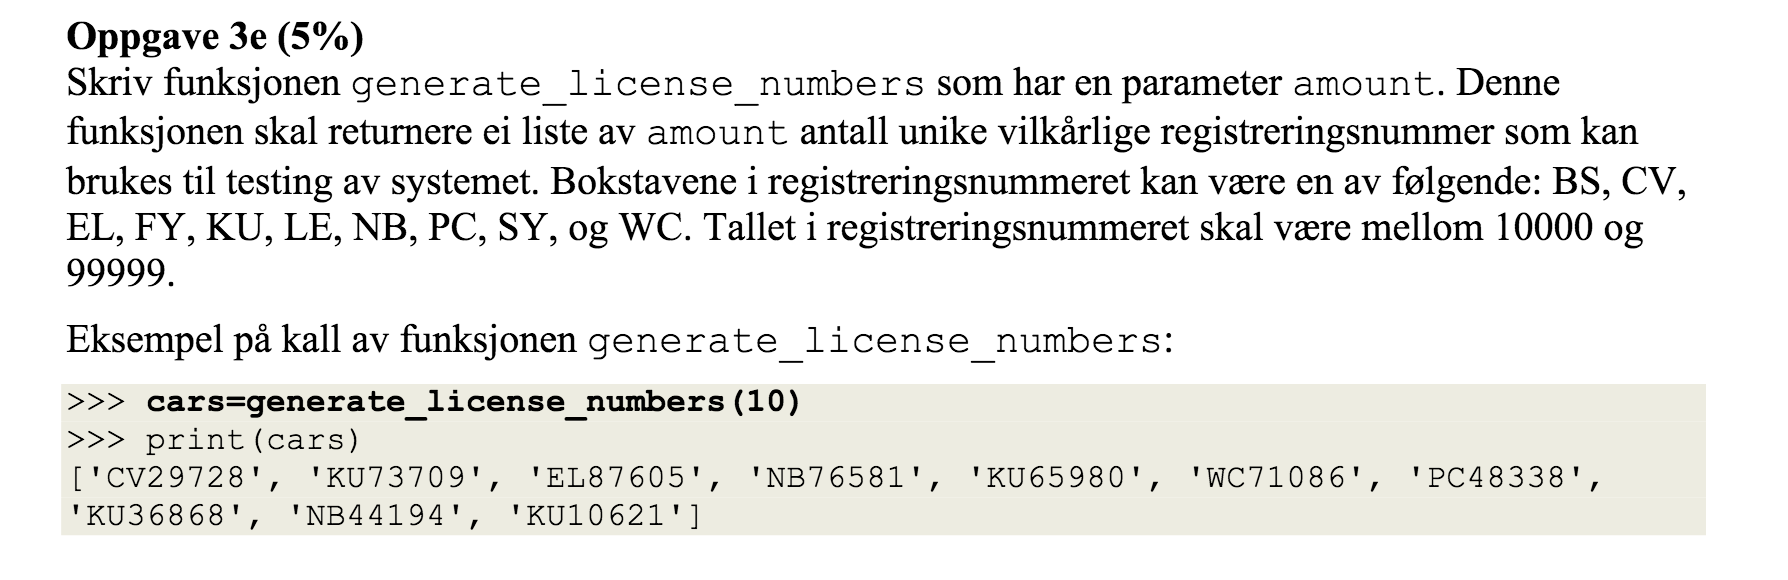
\includegraphics[width=\textwidth]{fig/streng_2017.png}
        \label{fig:my_label}
    \end{figure}
    
\end{frame}

\begin{frame}{Eksamensoppgave (2017H) (2)}
    \begin{figure}
        \centering
        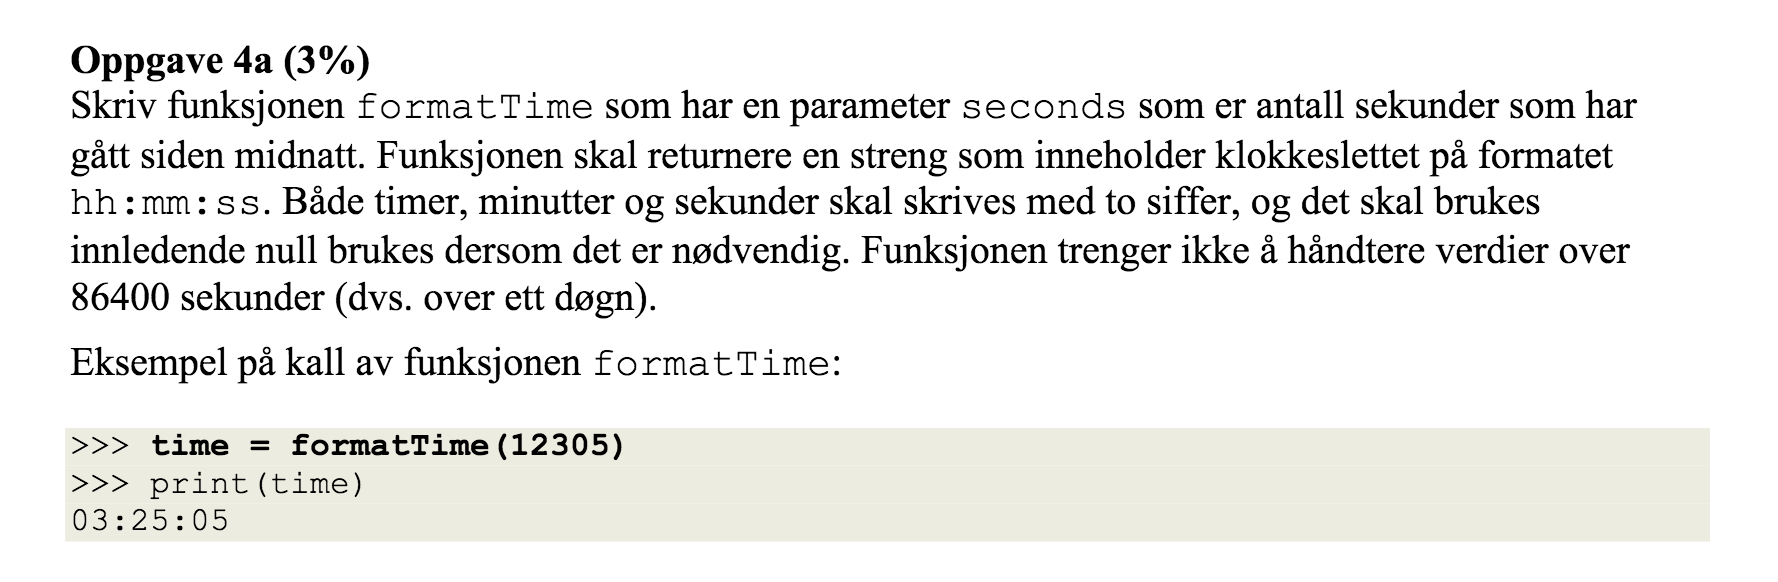
\includegraphics[width=\textwidth]{fig/time_2017.png}
        \label{fig:my_label}
    \end{figure}
    
\end{frame}

\begin{frame}{Oppgave 2: Yatzy - Utvidelse}
	\begin{itemize}
		\item<+-> Lag en funksjon som lager en liste med 5 tilfeldige heltall mellom 1 og 6 - (Gjorde vi sist)
	
		\item<+-> Lag en funksjon som tar inn en liste og en index som parameter og endrer tallet på indexen til et nytt tilfeldig tall, så returnerer listen

		\item<+-> Utvid funksjonen til å ta inn en liste med terninger og en \textbf{liste} med indexer og triller alle terningene på de gitte indexene på nytt

		\item<+->  Lag en funksjon som spør spilleren hvilke terninger han/hun vil trille om igjen via indexer, og returnerer en liste med indexene, det skal se ut som dette:
		\begin{itemize}
    \item   Hvilke terninger vil du kaste på ny? (separer med komma uten mellomrom – 1,3,5
    \end{itemize}
    \item<+-> Lag en funksjon fullfører alle tre kastene i et yatzy-kast og som spør hva som skal kastes på ny etter kast en og to
    \begin{itemize}
        \item Hint: indexer = nytt\_kast\_indexer()
	mitt\_kast = nytt\_kast(mitt\_kast,indexer)
	def kast():

    \end{itemize}

	\end{itemize}
\end{frame}



\begin{frame}{Spørsmål}
	\begin{itemize}
		\item Spørsmål kan også sendes på mail til \href{mailto::olemagnp@stud.ntnu.no}{olemagnp@stud.ntnu.no}
	\end{itemize}
\end{frame}

\end{document}
